\newlecture
\setcounter{chapter}{11}
\setcounter{section}{0}

\def\textbookchapter{Course Topic III: Multiple Integration}

%\def\textbookchapter{Chapter 11: Multiple Integrals}
\def\coursetopicnumber{III}
\def\topic{Double Riemann Sums and Double Integrals over Rectangles} % this is the printed title
\def\shorttopic{Double Riemann sums, integrals} % short topic
\def\textbookname{Active Calculus} % this is the corresponding textbook
\def\shorttextbookname{AC} % this is the short name for the book
\def\textbooksection{11.1} % corresponding textbook section
\def\textbooksectionurl{https://activecalculus.org/vector/S-11-1-Double-Integrals-Rectangles.html} % URL for textbook section
\def\handoutday{} % this is the printed date

\addtocontents{toc}{\bigskip \large \textbookchapter \normalsize \medskip \par} %% for table of contents
%%%%%%%%% DOCUMENT CONTENT STARTS BELOW

\thispagestyle{plain}
\topstuff
\section{\topic{} \booklink{}}
\label{sec:double-integral-rectangle}

\subsection{Integration in Calculus II}
The main result we need in this section is that the area of an $l\times w$ rectangle is %$l\cdot w$.
\bigskip 

\noindent In Calculus II, we saw the definite integral of a single-variable continuous function $f(x)$ on the interval $[a,b]$:
\[
    \int\limits_a^b f(x)\dx\hspace{3in}\mbox{}
\] 
%\vspace{.2in}

\noindent
\begin{minipage}{.5\textwidth}
    This gives us the signed area under the graph of $y=f(x)$ from $x=a$ to $x=b$. Here's how we evaluate it:
    \begin{itemize}
        \item Chop the interval $[a,b]$ up into $n$ subintervals $I_1, I_2, \dots, I_n$, each of width $\Delta x$ where
        
        \medskip 
        {\centering 
            $\Delta x=\phantom{\frac{b-a}{n}}$
        \par}%\hide{\frac{b-a}{n}}$
        
        \medskip 
        \item Pick a sample point in each subinterval. Call the sample points $x_1^*,\, x_2^*,\, \dots,\, x_n^*$.
        \item Draw rectangles in each subinterval with heights $f(x_1^*),\, f(x_2^*),\, \dots,\, f(x_n^*)$.
    \end{itemize}
\end{minipage}
\begin{itemize}
    \item Add up the areas of the rectangles. 
    
    \noindent Rectangle area = %\hide{f(x_1)\Delta x + f(x_2)\Delta x + \dots + f(x_n)\Delta x}$
    \vspace{.3in}
    
    \item In summation notation, the rectangle area is 
    % $\sum\limits_{k=1}^n f(x_k)\Delta x$.
    \vspace{.2in}
    
    \item There will probably be some error. If we use more rectangles, which will be narrower, we expect less error.
    \item If we let $n\to\infty$, the error will go to 0. In this case, the signed area under the graph of $y=f(x)$ from $x=a$ to $x=b$ is 
    %\[\lim\limits_{n\to\infty}\left(\sum\limits_{i=1}^n f(x_i^*)\Delta x\right)=\int\limits_a^b f(x)\dx.\]
\end{itemize}
%\end{minipage}
\vfill 

\pagebreak 

\subsection{Integration in Calculus III}
The main result we need now is that the volume of an $l\times w\times h$ rectangular box is % $l\cdot w\cdot h$.
\bigskip 

Now we think about a continuous function $f(x,y)$ and its graph $z=f(x,y)$ over a domain $R$ that is a rectangle in the $xy$-plane. This is a surface in $\mathbb{R}^3$. We'll be interested in the signed volume of the solid region under the graph of $z=f(x,y)$.

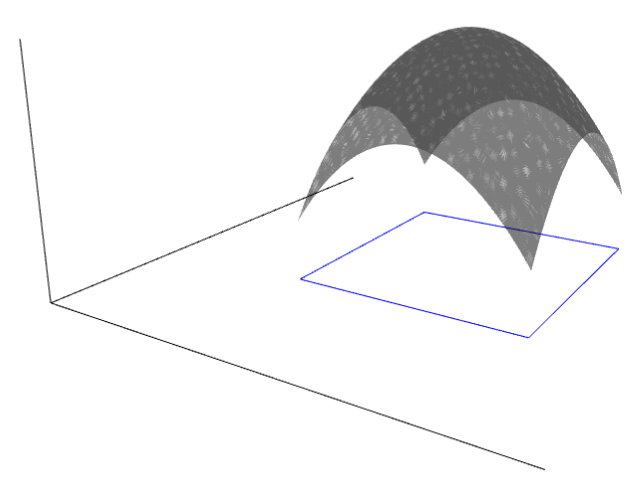
\includegraphics[width=.4\textwidth]{images/mesh1.png}\label{img:sage-double-int-1}

\begin{minipage}{.55\textwidth}
    For now, we'll focus on the rectangular region $[a,b]\times[c,d]$ in the $xy$-plane. In other words, points $(x,y)$ with $a\le x\le b$ and $c\le y\le d$ in the $xy$-plane. Just as we chopped up an interval into subintervals in Calculus I, we'll chop this rectangle up into subrectangles. Here's how we evaluate the signed volume.
    
    \begin{itemize}
        \item Chop the interval $[a,b]$ of $x$ values into $m$ intervals of width $\Delta x$. Thus 
        \[\Delta x = \hspace{1.5in} \] 
        %\frac{b-a}{m}$.
        %\medskip 
        
        \item Chop the interval $[c,d]$ of $y$ values into $n$ intervals of width $\Delta y$. Thus
        \[
            \Delta y = \hspace{1.5in} 
            \]
        %\frac{d-c}{n}$.
        %\medskip 
        
        \item Now we have $mn$ subrectangles which we list with double indices: 
        \[
            \left\{
                \begin{array}{cccc}
                    R_{1,1}, & R_{1,2}, & \dots, & R_{1,n}, \\
                    R_{2,1}, & R_{2,2}, & \dots, & R_{2,n}, \\
                    \vdots & \vdots & \ddots & \vdots \\
                    R_{m,1}, & R_{m,2}, & \dots, & R_{m,n}
                \end{array}
            \right.
        \]
        
        \item Each subrectangle has area $\Delta A = $%\Delta x \Delta y$.
        \item In each subrectangle $R_{i,j}$, pick a sample point $P_{i,j}=(x_{i,j}^*,y_{i,j}^*)$.
    \end{itemize}
\end{minipage}

\pagebreak 

\begin{itemize}
    \item Draw a rectangular box in each subrectangle $R_{i,j}$ with height $f(P_{i,j})$.
    \medskip 

    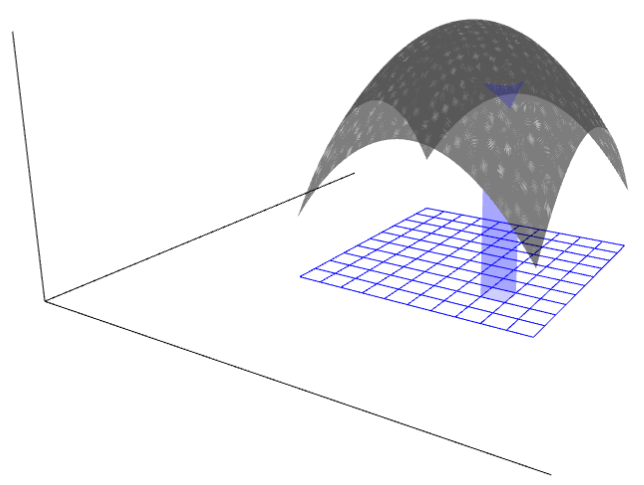
\includegraphics[width=.45\textwidth]{images/mesh2.png}\label{img:sage-double-int-2}
    \medskip 

    %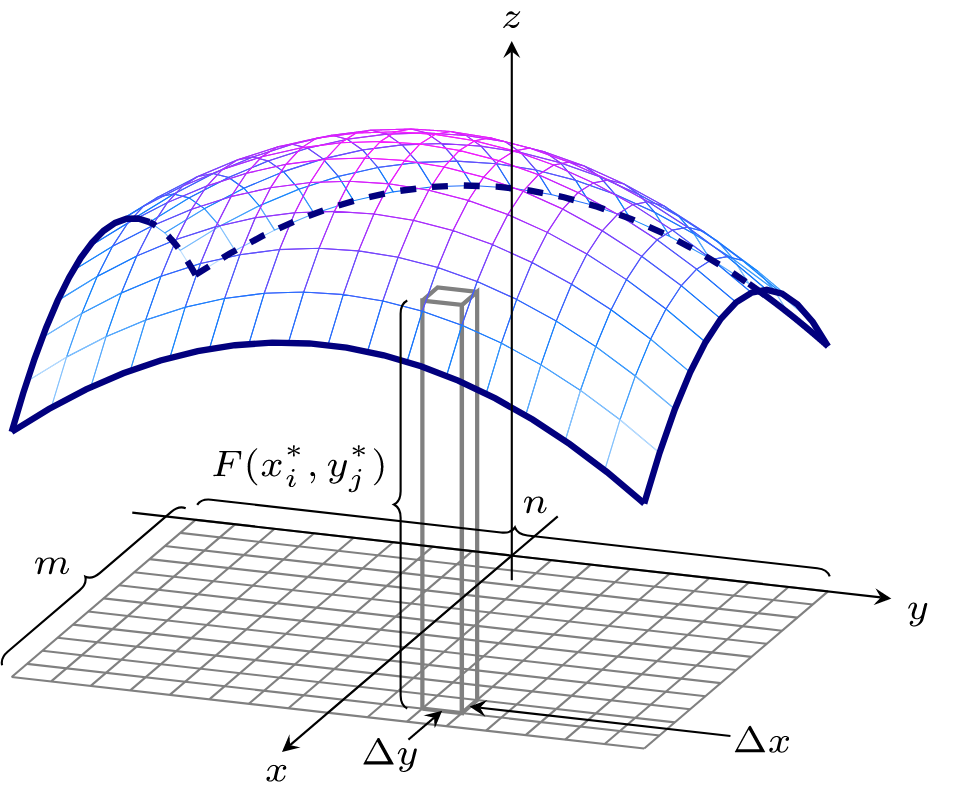
\includegraphics[width=.7\textwidth]{images/riemann2.png}\\
    \item The volume of the rectangular box above rectangle $R_{i,j}$ is % $f(P_{i,j})\delta A = f(x_i,y_j)\Delta A$.
    \item Add up the volumes of the rectangular boxes. \medskip 
    
    Rectangular box volume = $\left\{\begin{array}{cccc}
    f(P_{1,1})\Delta A &+ f(P_{1,2})\Delta A &+ \dots &+ f(P_{1,n})\Delta A \\ 
    +f(P_{2,1})\Delta A &+ f(P_{2,2})\Delta A &+ \dots &+ f(P_{2,n})\Delta A \\ 
    \vdots & \vdots & \ddots & \vdots \\ 
    +f(P_{m,1})\Delta A &+ f(P_{m,2})\Delta A &+ \dots &+f(P_{m,n})\Delta A.\end{array}\right.$
    \medskip 
    
    \item In summation notation, the rectangular box volume is
    %\[\sum\limits_{i=1}^m \sum\limits_{j=1}^n f(x_i^*,y_j^*)\Delta A.\]
    \vspace{1in}
    
    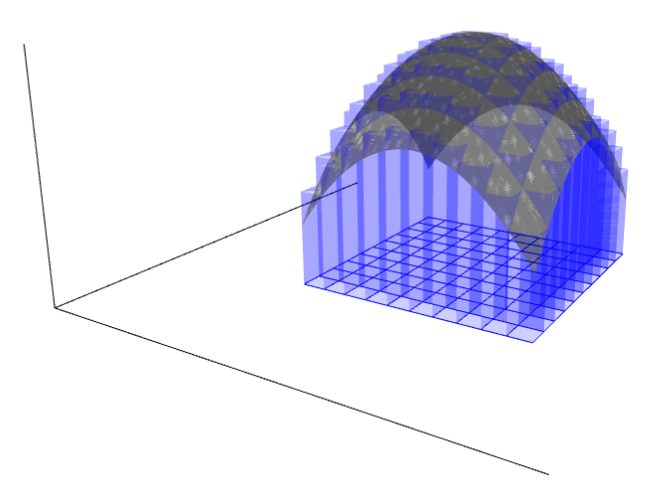
\includegraphics[width=.45\textwidth]{images/mesh3.png}
    \hfill 
    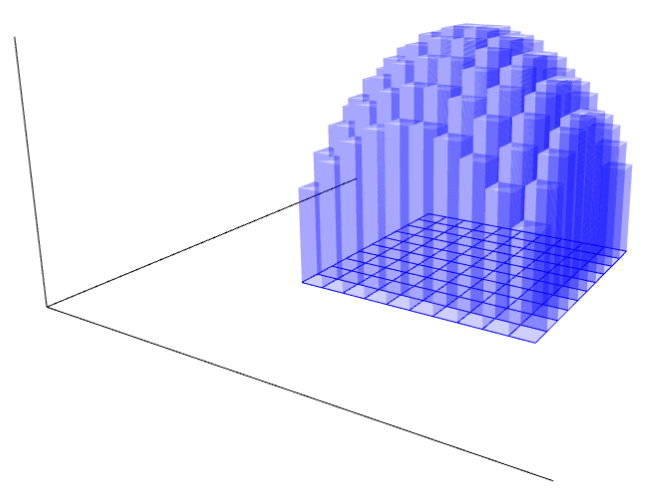
\includegraphics[width=.45\textwidth]{images/mesh4.png}
    
    \item There will probably be some error. If we use more rectangular boxes, which are then narrower in the $x$- and $y$-directions, we'll have less error.
    
    \pagebreak 
    
    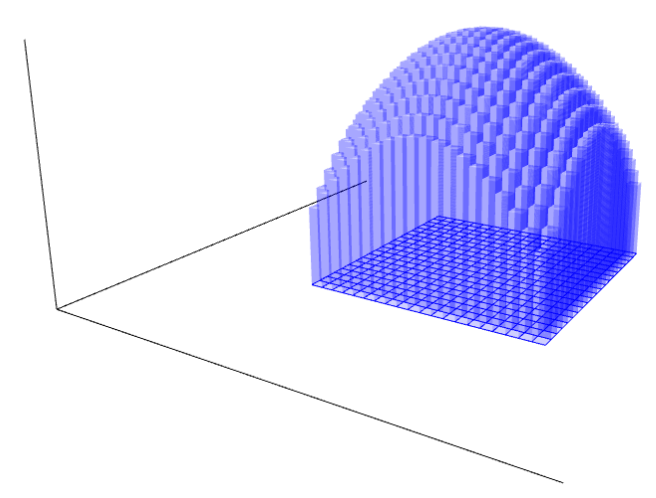
\includegraphics[width=.5\textwidth]{images/mesh5.png}\medskip \label{img:sage-double-int-3}
    
    \item If we let $m\to\infty$ and $n\to\infty$, the error will go to 0. In this case, the signed volume under the graph of $z=f(x,y)$ with $x$ from $a$ to $b$, and with $y$ from $c$ to $d$, is
    \[
        \phantom{\lim\limits_{m\to\infty}\lim\limits_{n\to\infty}\sum\limits_{i=1}^m\sum\limits_{j=1}^nf(x_{i,j}^*,y_{i,j}^*)\Delta A.}
    \]
\end{itemize}

\subsection{Double integral over a rectangle}
\begin{defn}[Double integral]
    In general, if we have a function $f(x,y)$ and want to find the (signed) volume under the graph of $z=f(x,y)$ over a rectangular region $R$ in the $xy$-plane, we write this as 
    \[
        \lim\limits_{m\to\infty}\lim\limits_{n\to\infty}\sum\limits_{i=1}^m\sum\limits_{j=1}^nf(x_{i,j}^*,y_{i,j}^*)\Delta A=\phantom{\iint\limits_R f(x,y)\dA.}
    \] 
    We call this the \emph{double integral of $f$ over $R$}.
\end{defn}

In Section \ref{sec:iterated-integration}, we will see how to evaluate a double integral over a rectangle $R$. In Sections \ref{sec:double-int-general-region} and \ref{sec:double-int-polar}, we will see how to evaluate double integrals over more general regions.
\bigskip 

\subsection{A first example}
We can occasionally use geometry to evaluate a double integral.

\begin{ex}\label{ex:double-integral-via-geometry}
    Let $f(x,y)=5$. For $R=[0,2]\times[1,4]$, evaluate $\iint\limits_R f\dA$.
\end{ex}

\vfill 

\pagebreak 

\subsection{Approximations}
In Calculus I/II, we primarily dealt with integrals in two ways: computing approximations via Riemann sums; and finding exact values via the Fundamental Theorem of Calculus.

In this course we will primarily focus on cases where we can obtain exact solutions for double integrals. Our primary tool is that of the \emph{iterated integral} which allows us to write a double integral as a combination of two single integrals, which we can then evaluate using methods from Calculus II. 

However, there may be times where we cannot get an exact value. When that occurs, approximation techniques like those from Calculus II can be used effectively. Here's an example.
\begin{ex}
    For the rectangle $R=[0,4]\times[-1,5]$, approximate the double integral $\iint\limits_R x^2y\dA$. Do so by subdividing $[0,4]$ up into $m=2$ subintervals, subdividing $[-1,5]$ into $n=3$ subintervals, and choosing sample points to be the midpoint of each rectangle.
\end{ex}

